
\begin{abstract}
Introduction of an automated  monitoring  system for test results on kidney function by way of statistical process control techniques needed evaluation for its effectiveness and impact. In order to gain confidence with the new system, doctors need to know that patients are getting the same or improved care, while funders would like to know that  additional costs are negligible, or are the result of extra services being applied to those patients with the greatest need and are therefore leading to improved health outcomes.

Treatment of patients whose renal function is low have high ongoing medical costs, especially once dialysis becomes the only remaining option for treatment. Introduction of a monitoring system would hopefully add value for the medical professionals taking care of patients whose condition is treatable in order to stave off the need for dialysis.
\end{abstract}

\pagebreak

\section{Introduction}

Kidney disease is an increasing problem worldwide. \citet{jha2013chronic}, described how practitioner awareness remains low despite the rising significance of renal disease. These authors argued that care would need to be led by primary care and integrated into general chronic condition management to avoid the ``catastrophic" costs associated with the management of advanced chronic renal disease management \citep{jha2013chronic}. 
The cost of renal disease was estimated  at 1.44-1-45 billion in 2009-2010 for the UK alone \citep{kerr2012estimating}. 


The system developed by \citet{GodfreyEtAl2014KidneyPaper} responded to the need to assist doctors and renal care specialists handle the deluge of data they had or were about to have if the concerns over a diabetes epidemic would come to pass. It was important to filter the results for patients in need of further monitoring from those patients with standard renal function, and then to determine if the monitoring regime was suitable for the patient's current situation. Concerns over the need to process a large quantity of test results is not novel; \citet{poon2004wish} reported that American primary care physicians spent 74 minutes per day reviewing results. Despite which 81\% reported delays in managing results and only 41\% were satisfied with their current process.

After a successful pilot testing phase using patients for four physicians, the system described by \citet{GodfreyEtAl2014KidneyPaper}  was deemed suitable for wider release; it was given a working name of `RenalQ' and was rolled out for all patients in the local District Health Board's catchment area. On 1 April 2015, all other systems related to the processing of kidney function test results were suspended, and to date have not been re-engaged. % is that date right? it feels wrong
During the first few months of operation the implementation team turned their attention to finding a means of evaluating the system to show other District Health Boards that they should implement the system in their areas. This paper outlines the methods used to illustrate the effectiveness of the RenalQ system and which patients are benefitting from RenalQ's implementation.
There are two main concerns to consider about the impact the introduction has had on the service provider. We ask the two questions: \begin{enumerate}
\item Has RenalQ led to an increase in total testing numbers?
\item Have the patients whose condition with respect to renal function had a change in the frequency over which they are being tested? 
\end{enumerate}
Ultimately we would hope that the answer to the first question is either ``no", or that if it is ``yes", that the increased amount of testing is being directed to those patients who would be considered in need of greater monitoring in order to achieve improved health outcomes.

In Section~\ref{TheSystem} we briefly outline the RenalQ	 system, while Section~\ref{Methodology} gives details of the data and methodology used to evaluate the implementation of RenalQ. We present and discuss our findings in Section~\ref{Findings} and offer some conclusions in Section~\ref{Conclusions}.

\section{The System}  \label{TheSystem} 

A patient's Glomerular Filtration Rate (GFR) can be estimated  following  a serum creatinine test taken in a clinical laboratory as part of a standard blood test. RenalQ pulls the historical data for a patient using their unique identifier attached to the digital request identifier for the blood test and then compares the current test result with the historical data. The analysis depends on the length of a patient's history of testing; if the history is short, then RenalQ will recommend a timeframe for the next test depending on the level of the patient's eGFR and recent data history. The rules used by RenalQ in these circumstances are aimed at increasing the amount of testing for patients whose eGFR is well below average for a patient in good health, while a patient who is above average is in no need of further testing at this time.
 
Patients will therefore build a history of eGFR results over time, with those most in need of ongoing monitoring building a history faster than patients in good health. If a patient moves from good health as indicated by a lower eGFR, they will have a new recommendation based on their current condition. It is likely therefore that patients with a longer history of eGFR test results will be those patients who are in the greatest need of monitoring.

For those patients who have a long history of eGFR results, RenalQ uses statistical process control techniques to evaluate the latest test result in the context of each patient's history. Each patient's data is then evaluated using three control charts: a standard control chart for individual observations, an exponential weighted moving average chart, and a CUSUM chart. This set of graphical displays is created for clinicians to consider, but RenalQ offers a recommendation based on a number of decision criteria in common use with these control charts; a more complete discussion of the control charts and associated decision criteria can be found in \citet{GodfreyEtAl2014KidneyPaper}. Each decision criterion is a warning that something unusual is happening for the patient; these warnings are set at fairly conservative levels which trigger a change in the recommended time to the next test being sought. In other words, the patient's recommended time to their next test remains as it was before the last test unless something has changed for that patient. This trigger is then a signal to the patient's physician that they ought to take a special interest in their patient following the latest test. Physicians can also see that the recommended course of action has not changed for their patient; they can of course use their professional judgement to override any recommendation that RenalQ has provided.

\citet{GodfreyEtAl2014KidneyPaper}  proposed that RenalQ has the potential to direct the attention of clinicians and physicians to the patients that have the greatest need. RenalQ may increase the total amount of testing that is sought because it is conservative, especially for those patients with below average renal function. The challenge is to determine if in fact this cost is offset by sufficient improved health outcomes for the individual patients and wider population as well as benefits in resource allocation of increasingly limited human resources and capital equipment. .

\section{Methodology} \label{Methodology} 

We have extracted the entire dataset of eGFR test results for our District Health Board from 1 January 2012 to 31 March 2016 for evaluation. RenalQ went totally live on 1 April 2015 so we have 3.25 years of data to use as a baseline against which RenalQ's impact will be gauged. We are able to compare the total number of tests being conducted over time, and ascertain if any change in the total number of tests is being affected following the introduction of RenalQ.  
The provided data file contained  a total of 255,567  renal function test results conducted during the period starting 2 January, 2013 until 31 March, 2016; these tests were  for a total of 92,735 patients. We wish to question the totality of results;  the results from 2013 may be incomplete because we were provided with data that showed very low numbers of results from 2012, and we do not know when the provided data started to incorporate every test being conducted.


For the purposes of evaluating the time until the next RenalQ test is performed on each patient, we removed all patients who were under 18 years old and the pregnant women as these patients were not subjected to analysis via RenalQ. We also removed the patients whose age or sex was not provided. This allows comparison of the patient results for the RenalQ system with those obtained before RenalQ was introduced. 
This leaves 246,824  test records for 87,316   patients.


In addition to the impact on the total workload for testing, we are interested in what is happening for individual patients following the introduction of RenalQ. 
We have searched through our data to see when the next test following each test for individual patients was conducted.  We can therefore evaluate the number of days between tests against a number of factors including the patient's age, gender, and the current test result.
Many patients will appear only once in our data as they either have only one test ever, or any other tests they may have had occurred before 1/1/12 or after 31/3/16. We are not particularly concerned with any test result prior to 1/1/12, but there is an impact on how we ought to evaluate the recommendation process offered by RenalQ if a patient has not yet returned for another test. The time to the next test for these patients is therefore recorded as the number of days until 1/4/16, but we note that it is `censored' data as the next test date remains unknown. Every patient therefore has one censored observation within the data set. We ignored the approximately 3500 records that did not have an NHI number attached as these were for work done under exceptional circumstances and not for management of patients within the intended catchment population.


Censored data is commonly found in the evaluation of medical treatments or product testing scenarios where the study period comes to an end without the phenomenon of interest occurring for some experimental units. The appropriate statistical tools for this data scenario are commonly referred to as survival analysis; the survival analysis technique of most interest in our evaluation of RenalQ is  regression for censored data.

All analyses have been conducted using the R statistical application \citep{RItself} and the following additional packages: data.table \citep{data.tablePkg} for data importing and handling of large files; dplyr \citep{dplyrPkg} for data manipulation and some calculations; lattice \citep{latticePkg} for plotting figures; lubridate \citep{lubridatePkg} for processing of date/time data; qcc \citep{qccPkg} for creation of control charts; and survival \citep{survivalPkg} for the statistical analysis of time to event data.

\section{Findings} \label{Findings} 


\subsection{Analysis of total testing workload}



We limit our investigation of the total amount of testing being conducted to the last 39 months from January 2013 to March 2016.

\includegraphics{Figures/Monthly-TSPlot}


There is a (perhaps not so obvious) pattern in this data to draw to the reader's attention. It seems both a seasonal effect over the months within a year, and a general increase over years should be noted.  Our belief in this notion is supported by use of an Analysis of Variance (ANOVA) procedure.


\begin{Schunk}
\begin{Soutput}
Analysis of Variance Table

Response: n
                 Df  Sum Sq Mean Sq F value    Pr(>F)    
as.numeric(Year)  1 4961349 4961349 54.1576 1.339e-07 ***
Year              2  223442  111721  1.2195 0.3130261    
Month            11 5773449  524859  5.7293 0.0001773 ***
Residuals        24 2198628   91609                      
---
Signif. codes:  0 '***' 0.001 '**' 0.01 '*' 0.05 '.' 0.1 ' ' 1
\end{Soutput}
\end{Schunk}



The above table shows that the impact of year can be summarised as a straight line effect, while we have a cyclic pattern over the months. Any departure from this would constitute an unusual increase in total workload since the introduction of RenalQ. We use a standard control chart for individuals to search for unusual results. The control limits on the plot are calculated using the data from before the introduction of RenalQ and are at two (shown in orange) and three (shown in red) standard deviations from the centre line.

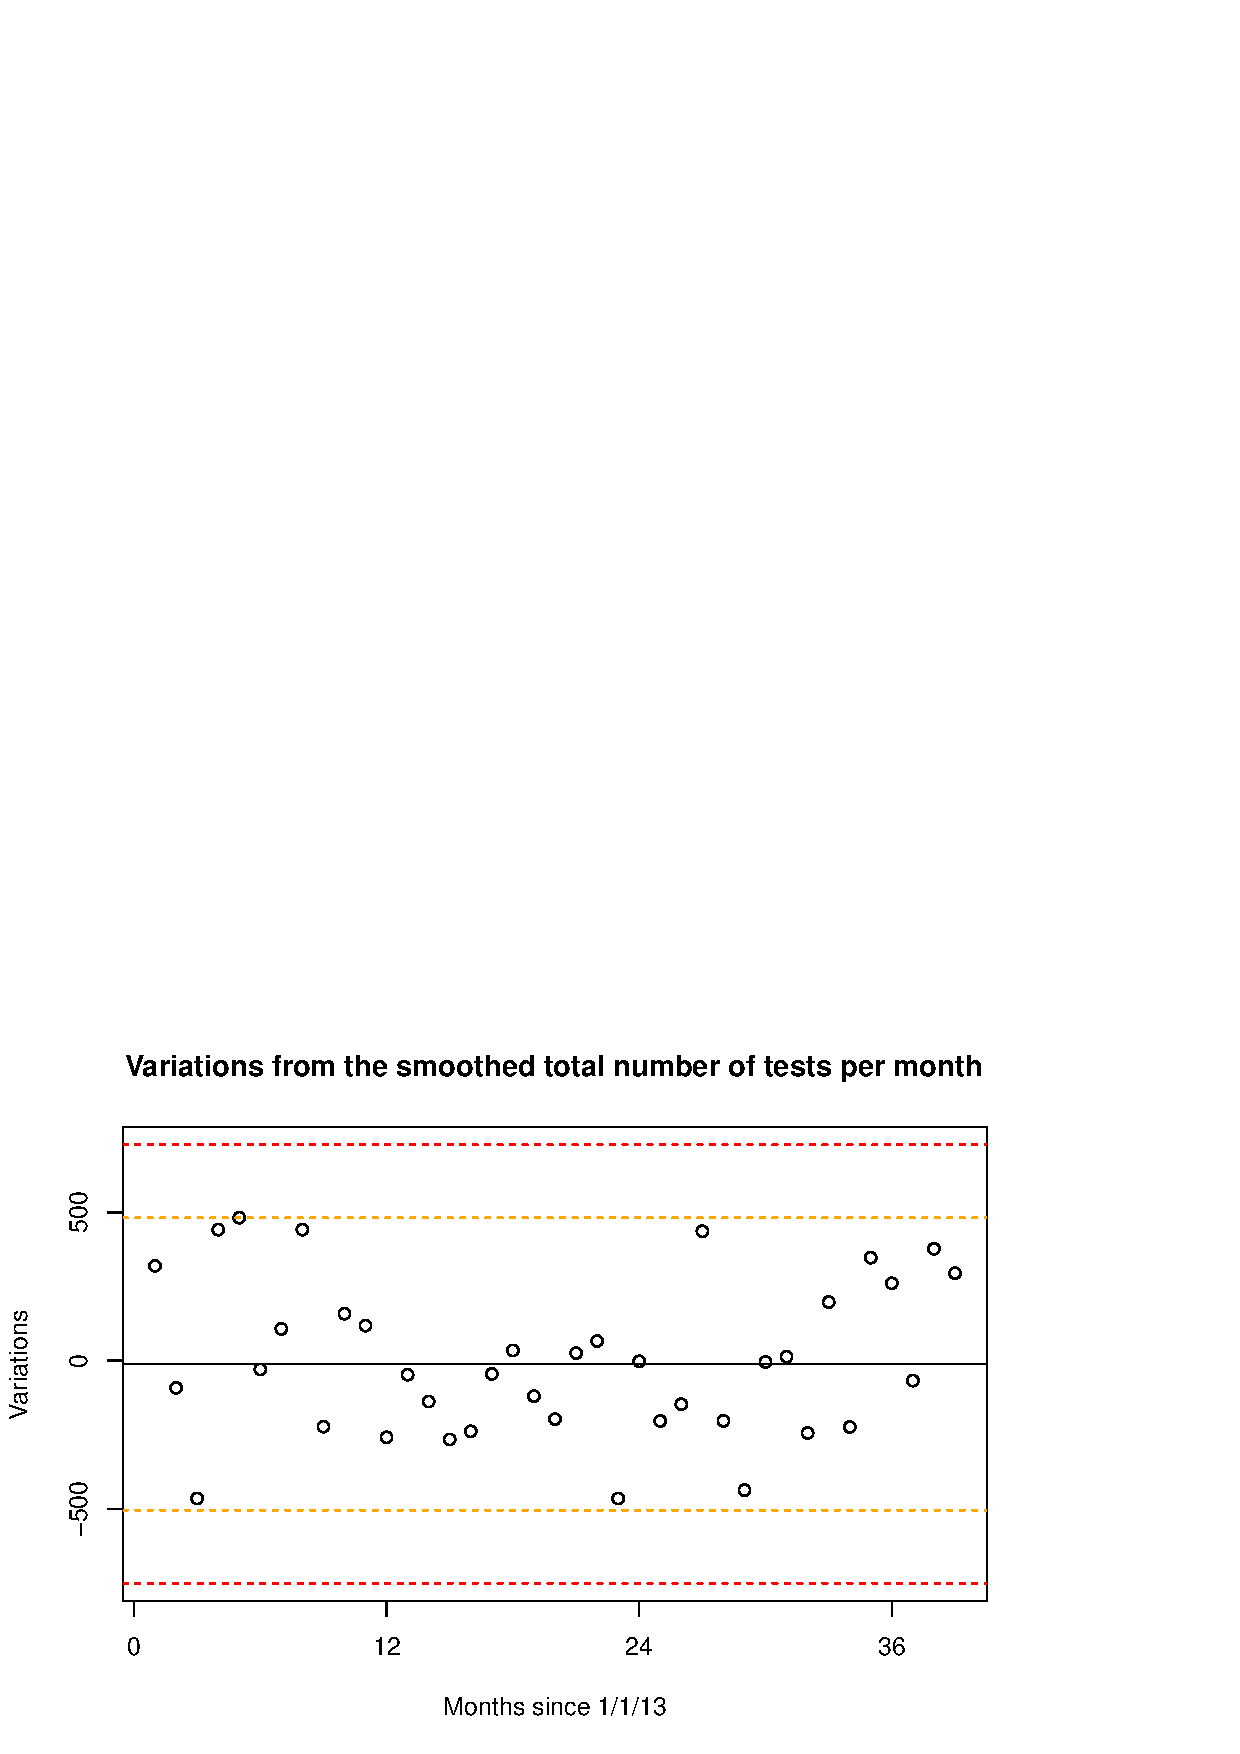
\includegraphics{Figures/Monthly-QCC}

There are no serious  departures (outside three standard deviation limits) from what could be expected in terms of the total number of tests being conducted. We do need to condition this assessment on our concern that the totality of tests has not been provided for earlier years of this investigation. This aspect of this report can be re-created once the reliability of the complete data can be established.




Even though the total number of tests is growing, it is worth seeing if the mix of tests is changing at all. We have used a $\chi^2$ test to see if the counts of tests yielding different eGFR values is changing over time. The eGFR values have been put into five categories using cut-offs of 15, 30, 60, and 90

\begin{Schunk}
\begin{Soutput}
'data.frame':	195 obs. of  5 variables:
 $ X     : Factor w/ 195 levels "1","10","100",..: 1 108 119 130 141 152 163 174 185 2 ...
 $ Year  : Factor w/ 4 levels "2013","2014",..: 1 1 1 1 1 1 1 1 1 1 ...
 $ Month : Factor w/ 12 levels "1","10","11",..: 1 1 1 1 1 5 5 5 5 5 ...
 $ EGFR_G: Factor w/ 5 levels "(-1,15]","(15,30]",..: 1 2 3 4 5 1 2 3 4 5 ...
 $ n     : num  37 193 1073 2690 1838 ...
\end{Soutput}
\end{Schunk}

The test has a $\chi^2$ value of 3175.89 (p=0, df=152) which means there is a change in the pattern of testing over time for the five categories.

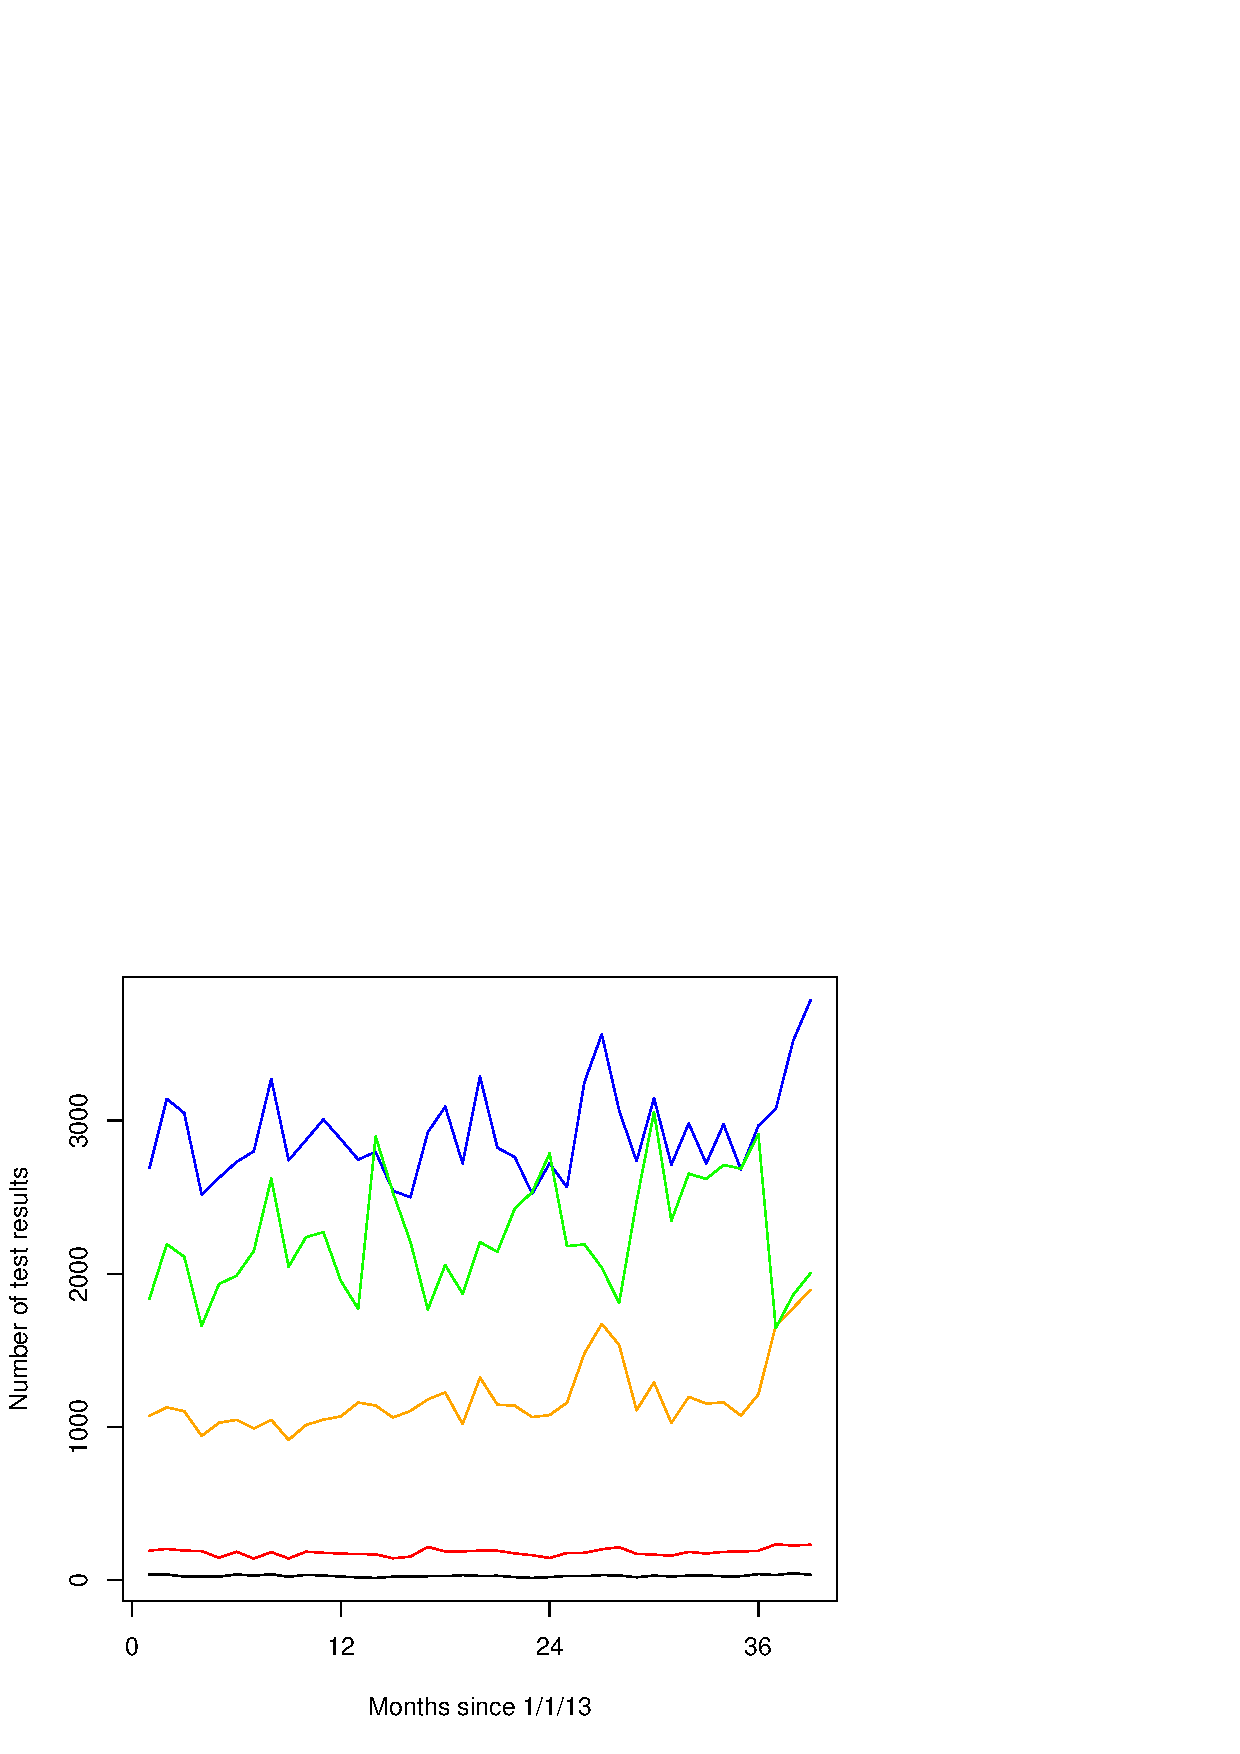
\includegraphics{Figures/Monthly-LinePlots}

It is difficult to see any growth in the number of tests being conducted for patients whose eGFR is between 60 and 90 (shown in blue) and above 90 (shown in green). The patinet groups of greatest interest are those with eGFR between 30 and 60 (shown in orange) and between 15 and 30 (shown in red). The numbers of tests being conducted for patients with eGFR below 15 (shown in black) are extremely low and are probably not worth further analysis given how little they contribute to  the total testing workload. 



\subsection{Evaluation of the times between tests}


There is a substantial amount of data available for evaluation. Fitting a model to the entire set of data has proven difficult due to computer infrastructure limitations. The first analysis below allows for the differences among age groups and compares males with females, while the subsequent analysis  ignores these differences among the patients.

We have needed to group eGFR values and remove the 2013 data to accommodate the inclusion of sex and age group factors in the following analysis.



We have chosen to truncate the eGFR values at 100 for the purposes of this analysis. All patients whose eGFR is above 90 are said to be above average and showing no signs of renal dysfunction. We have also truncated at the critical end of eGFR by raising all eGFR values less than 10 up to 10; this decision has been taken due to the low number of patients that have such low eGFR values.

The model  used to identify the statistically significant factors affecting the time between successive renal function tests allows for each patient's gender (F or M), their age (Four categories), their level of renal function (as measured by their eGFR), and whether that test was analysed using the RenalQ system. In addition, the combination of many of these effects has also been incorporated in the model. The regression model for this model yields  the following summary of effects and their statistical significance.
\begin{Schunk}
\begin{Soutput}
                            Df     Deviance Resid. Df   -2*LL      Pr(>Chi)
NULL                        NA           NA    175141 1385851            NA
AgeGroup                   813 2.004357e+04    174328 1365808  0.000000e+00
SEX                          1 1.003970e+01    174327 1365798  1.532021e-03
System                       1 1.483301e+01    174326 1365783  1.174615e-04
EGFR_C                       9 9.598082e+03    174317 1356185  0.000000e+00
AgeGroup:SEX                 3 9.776814e+01    174314 1356087  4.691734e-21
AgeGroup:System              3 7.175265e+01    174311 1356015  1.798459e-15
SEX:System                   1 1.463972e-01    174310 1356015  7.020024e-01
AgeGroup:EGFR_C             27 8.486214e+02    174283 1355167 2.239113e-161
SEX:EGFR_C                   9 6.613466e+01    174274 1355100  8.674873e-11
System:EGFR_C                9 3.612780e+02    174265 1354739  2.461055e-72
AgeGroup:SEX:System          3 2.419292e+00    174262 1354737  4.900535e-01
AgeGroup:SEX:EGFR_C         27 6.430043e+01    174235 1354672  7.010564e-05
AgeGroup:System:EGFR_C      27 7.671858e+01    174208 1354596  1.174889e-06
SEX:System:EGFR_C            9 3.716795e+01    174199 1354559  2.456257e-05
AgeGroup:SEX:System:EGFR_C  27 4.459772e+01    174172 1354514  1.792207e-02
\end{Soutput}
\end{Schunk}
Most of the factors and their combined effects are statistically significant. Many of these differences are  quite small however. We have chosen to present the findings using a series of graphs. Each panel in the following figure uses the log (base 10) transformation on the number of days between tests. The vertical axis of each panel is therefore presented on the log scale and is marked with powers of 10 and while the numbers $10^2=100$ days and $10^3=1000$ days might be familiar, the reader should note that $10^{1.5}$ is approximately 31.62 days, while $10^{2.5}$ is approximately 316.23 days. The horizontal axis for each panel is the eGFR score for a test and there are two sets of points marked inside each panel. The pink coloured points show the number of days until the next test for given levels of eGFR following the introduction of RenalQ; the blue dots are the expected times to retest that were occurring before RenalQ was in operation. The eight panels are for the female (left) and male (right) patients while the four different age groups are presented vertically with the older patients at the top and the youngest at the bottom.

\includegraphics{Figures/Retest-ThePlots}

We would hope that the pink points lie below the blue ones for the range of eGFR values where we want patients to have increased monitoring, and above the blue ones for those patients who need less monitoring. The above plots indicate that when a  difference is noticeable, the difference suggest RenalQ is increasing the monitoring of patients showing poor renal function but no increase in monitoring of those patients whose renal function is above 60.



In the following analysis, the data for 2013 has been added back in and we have evaluated every value of eGFR instead of grouped eGFR values.




The next  model  used to identify the statistically significant factors affecting the time between successive renal function tests allows for only the level of renal function for each patient (as measured by their eGFR), and whether that test was analysed using the RenalQ system. In addition, the combination of these two effects has also been incorporated in the model. The regression model for this model yields  the following summary of effects and their statistical significance.
\begin{Schunk}
\begin{Soutput}
              Df    Deviance Resid. Df   -2*LL     Pr(>Chi)
NULL          NA          NA    246822 2250810           NA
System         1    81.24251    246821 2250729 1.996505e-19
EGFR_F        90 33987.39123    246731 2216742 0.000000e+00
System:EGFR_F 90   718.20686    246641 2216023 1.273500e-98
\end{Soutput}
\end{Schunk}


\includegraphics{Figures/RetestAll-ThePlots}

% This shows.


\section{Conclusions} \label{Conclusions}

We have investigated the two aspects that best show the impact of introducing the RenalQ system. First, we found that the total counts of tests being conducted  per month since the introduction of RenalQ are in line with the workloads that would have been expected  even if RenalQ had not been introduced. We have chosen not to show the breakdown of age groups and males versus females in this part of the analysis because we do not observe any unexpected increase. The fact that some increase does exist may need further investigation, but it is unreasonable to conclude at this time that this increase is due to the introduction of RenalQ.

One key aspect of RenalQ is the recommendation for the timing until a patient should get their next renal function test. If RenalQ is helping doctors increase the monitoring of patients with some degree of renal failure, the time to the next test should be decreasing. We see that in fact this is what is happening for those patients whose medical situation is in the critical phase where cheaper and less intrusive medical interventions can be offered.  Patients whose renal function has decreased to extremely low levels were being monitored successfully before the introduction of RenalQ; no material impact has resulted for these patients.

 
